\chapter{State of the art}
\label{chap: sota}


\section{Videospiel-Markt}
\label{chap: sota videospielmarkt}

Videospiele sind Bestandteil des Medienkonsums in Deutschland. Rund 6 von 10 Menschen in Deutschland spielen Computer- und Videospiele. Der deutsche Videospiel-Markt machte mit Videospiel-Hardware, Videospiel-Abo-Diensten und Videospielen im Jahr 2023 einen Umsatz von 9,97 Milliarden Euro. Dabei machten Videospiele und In-Game K\"{a}ufe mit 5,845 Milliarden Euro einen Umsatz von ca. 59\% aus. Im Vorjahr 2022 entstand ein Umsatz von 9,432 Milliarden Euro, somit stieg der Umsatz von 2022 im Jahr 2023 um 6\%.  Zahlen f\"{u}r das Jahr 2024 sind noch nicht bekannt.

\begin{figure}[h]
  \centering
  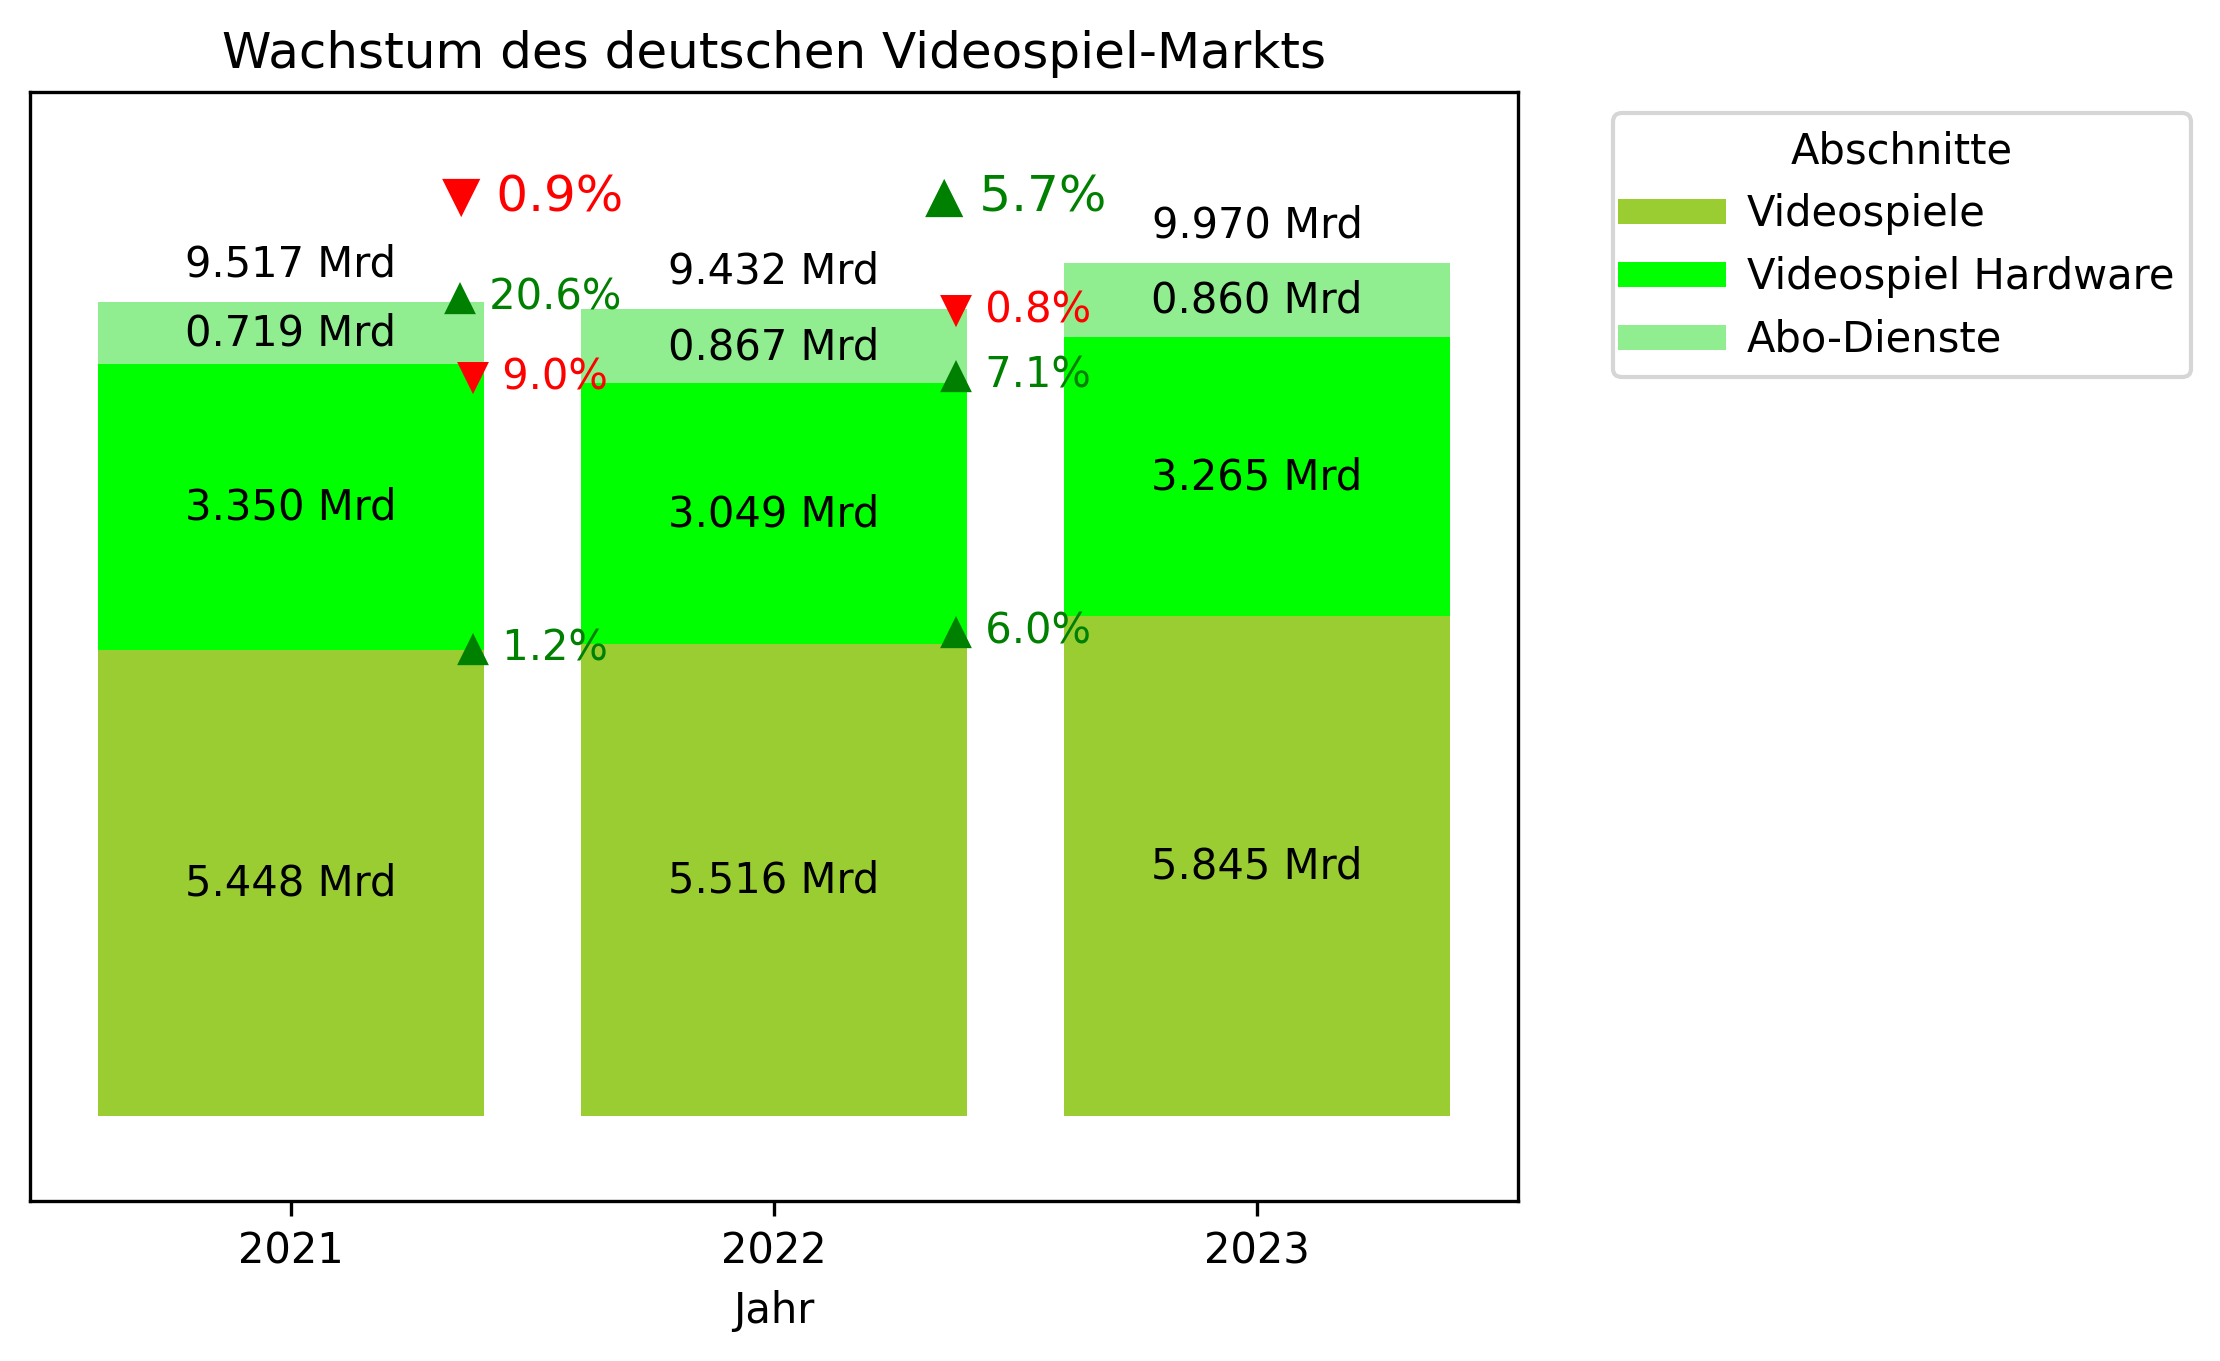
\includegraphics[width=15cm]{state_of_the_art/deutscher_vs_markt}
	\captionsetup{justification=justified, format=plain}
  \caption{Wachstum des deutschen Videospielmarkts \"{u}ber die Jahre}
  \label{Deutscher Videospielmarkt}
\end{figure}

Auf der erfolgreichen Computerspiel Vertriebsplattform Steam von Valve wurden vergangenes Jahr 2023 14.324 Computerspiele ver\"{o}ffentlicht. Seit 2019 w\"{a}chst die Ver\"{o}ffentlichung der Computerspiele auf Steam stetig.

\begin{figure}[h]
  \centering
  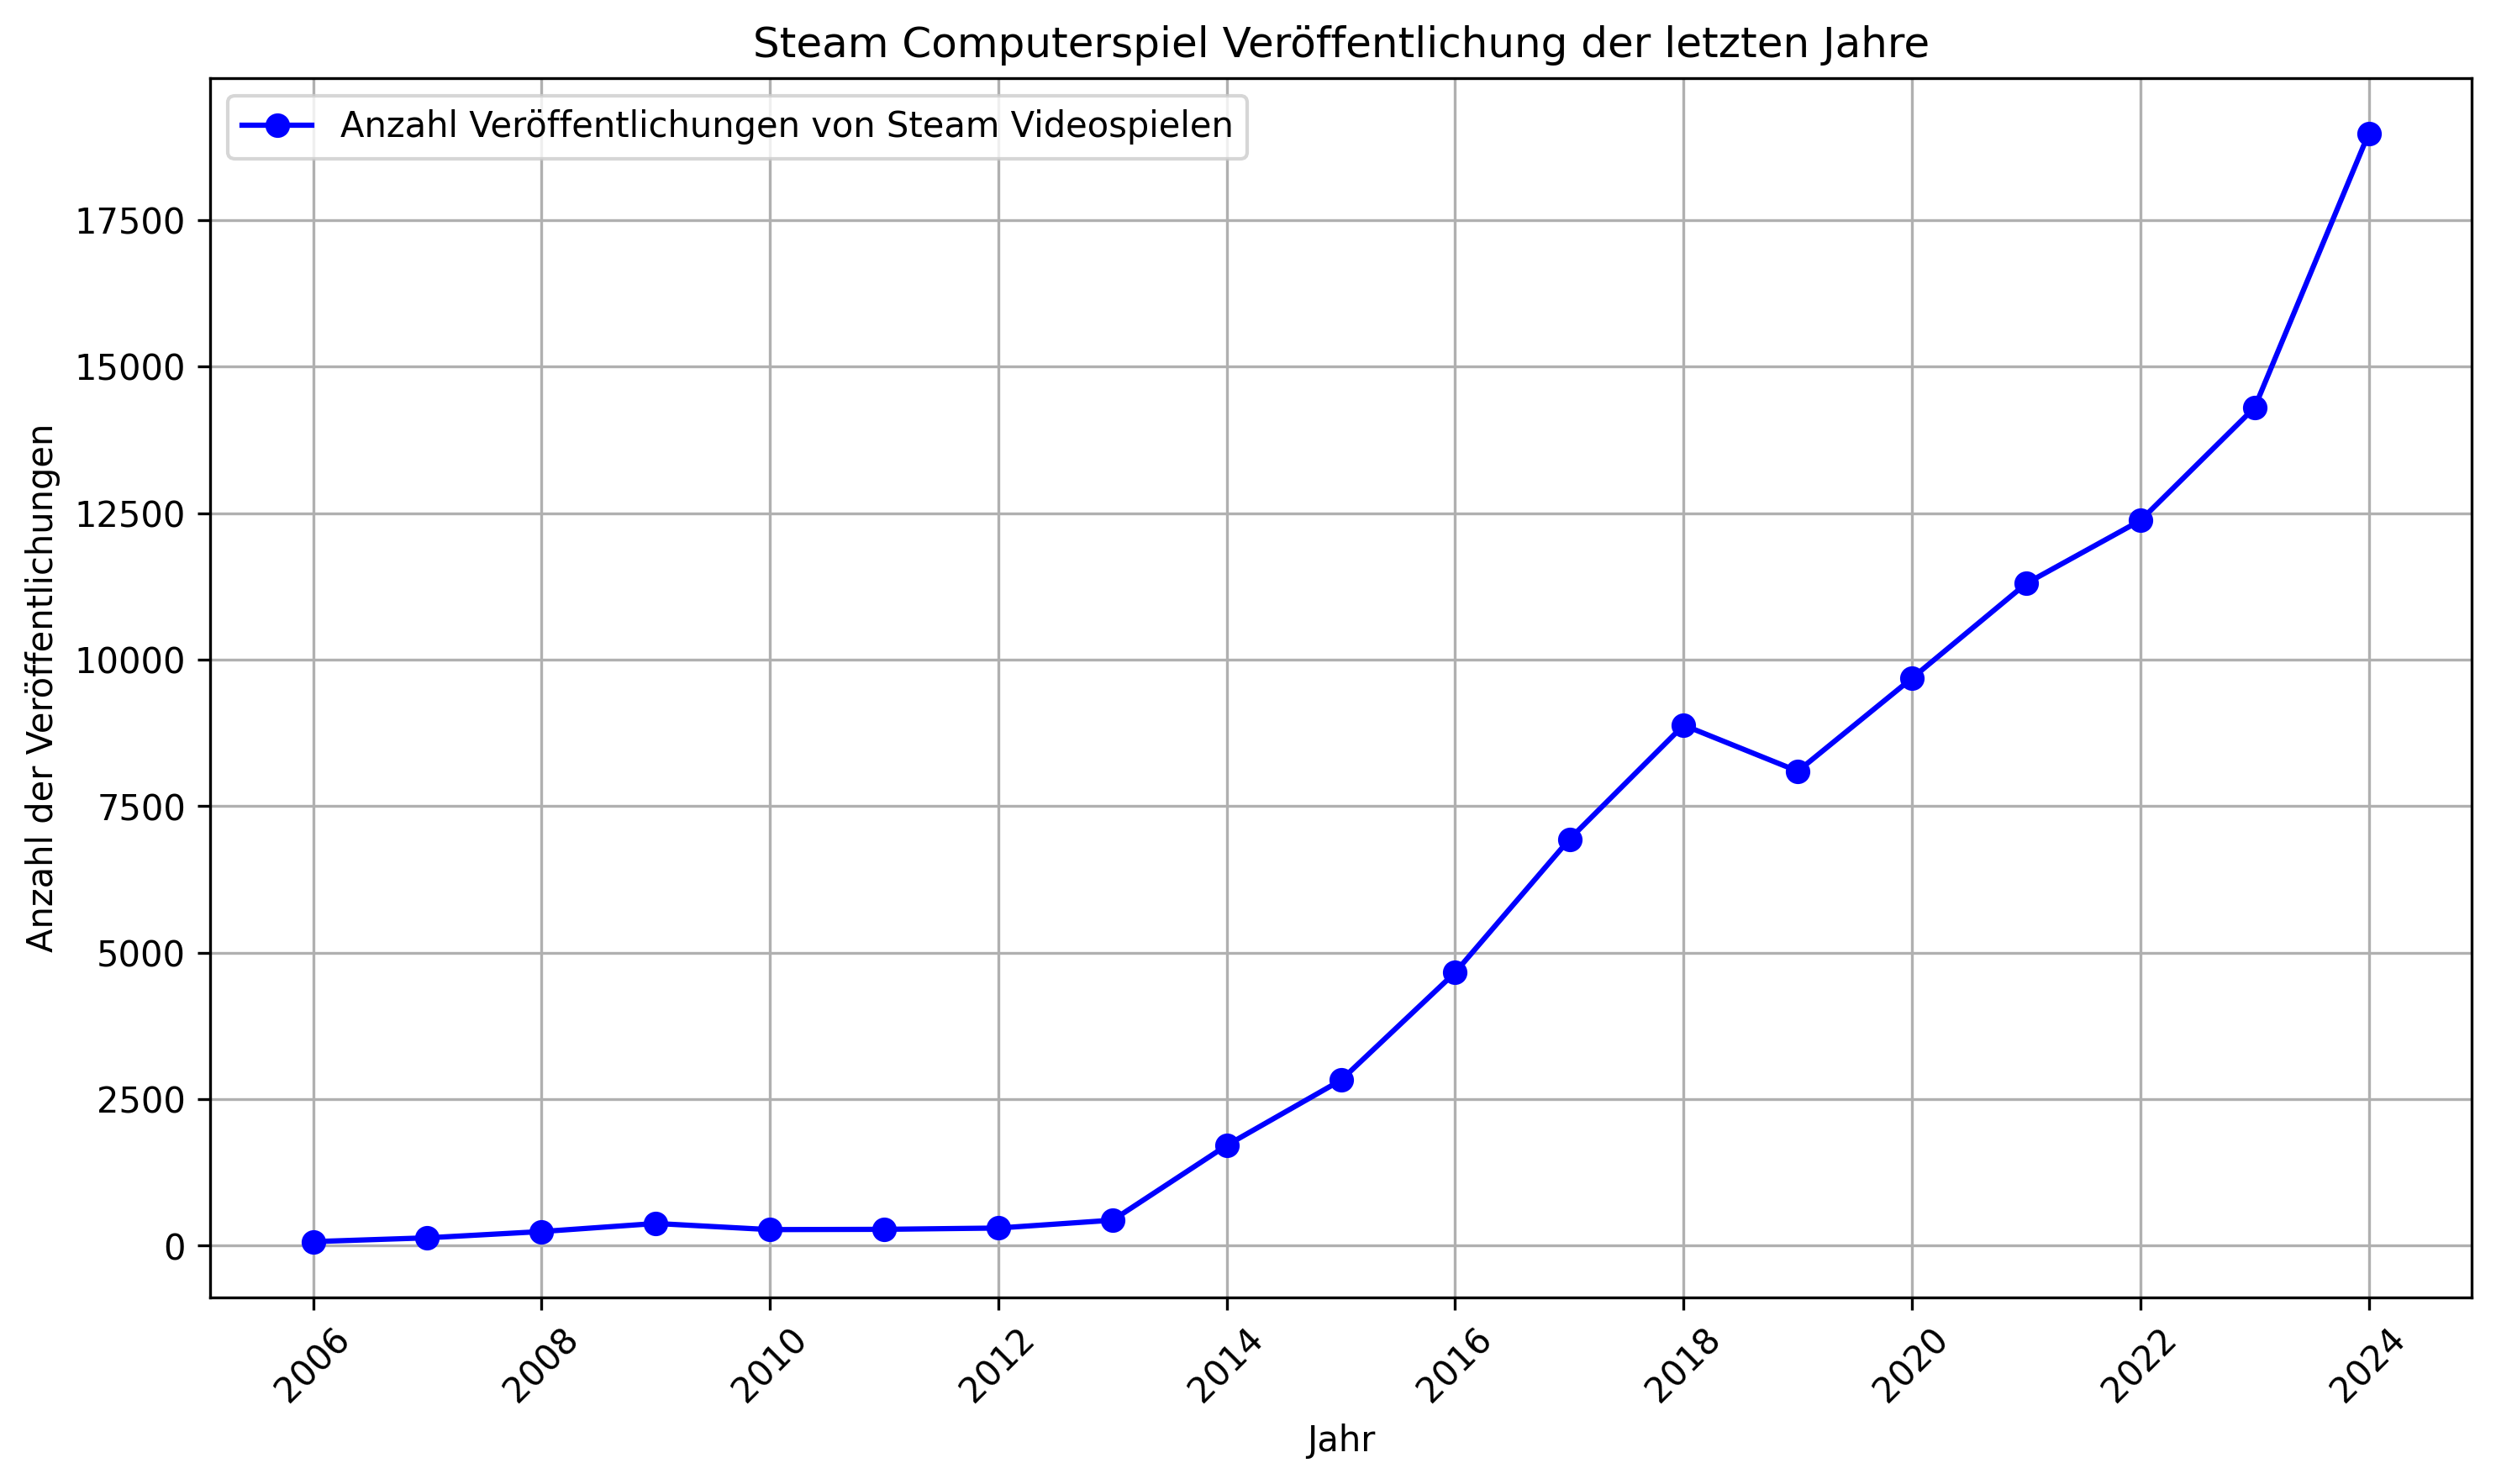
\includegraphics[width=15cm]{state_of_the_art/steam_veroffentlichungen}
	\captionsetup{justification=justified, format=plain}
  \caption{Computerspiel Ver\"{o}ffentlichungen auf Steam \"{u}ber die Jahre}
  \label{SteamDB Statistik}
\end{figure}

Folglich kann davon ausgegangen werden, dass es Stakeholder gibt, die sich f\"{u}r Videospiele interessieren.



\section{Game-Engines}
\label{chap:sota game-engines}

Seit der Doom-Engine sind neue \hyperref[chap:game engines]{Game-Engines} entstanden und haben sich weiterentwickelt. Zu den g\"{a}ngigen zug\"{a}nglichen Game-Engines geh\"{o}ren: Unreal-Engine, Unity und Godot. Godot ist dabei die j\"{u}ngste Game-Engine und konkurriert mit der Unity. In den letzten Jahren hat Unity das Vertrauen von Entwicklerstudios verloren. Viele Entwicklerstudios wechseln nun in den letzten Jahren ihre Game-Engine. Das folgende Teilkapitel wird den derzeitgen Stand von den drei Game-Engines beschreiben.  

%Gro\ss{}e Entwicklerstudios besitzen ihre eigene Game-Engine. So nutzt beispielsweise das deutsche Entwicklerstudio Crytek die Cryengine. Eine eigene Game-Engine zu entwickeln ben\"{o}tigt zus\"{a}tzliche Ressourcen. Dagegen ist dies bei Indie-Entwicklerstudios schwer umsetzbar. Denn sie haben weniger Arbeitskr\"{a}fte als gro\ss{}e Entwicklerstudios und entwickeln Videospiele ohne finanzielle Unterst\"{u}tzung gr\"{o}\ss{}erer Unternehmen. Dadurch sind Indiestudios von m\"{o}glichst kosteng\"{u}nstigen Game-Engines abh\"{a}ngig.\autocite{holfeld2024relevancegodotengineindie}

\subsection{Unity}
\label{chap:sota unity}

Unitys Versuch, ein neues Geb\"{u}hrenmodell f\"{u}r Entwickler einzuf\"{u}hren, hat die Wahrnehmung der \hyperref[chap:game engines]{Game-Engine} als entwickler-freundliches Programm negativ beeinflusst. So k\"{u}ndigte Unity September 2023 eine \"{A}nderung des Geb\"{u}hrenmodells, zum Anfang des Jahres 2024, an. Die neue Regelung sah vor, dass Entwickler ab einem Umsatz von 200.000 US-Dollar und mindestens 200.000 Installationen f\"{u}r jede Erstinstallation eines Spiels 20 US-Cent an Unity zahlen sollen.\autocite{golem1}

Die \"{A}nderung h\"{a}tte finanzielle Folgen f\"{u}r viele Entwicklerstudios, insbesondere f\"{u}r Indieentwickler. Videospielentwickler sprachen davon, dass Unity sie in den Bankrott treiben w\"{u}rden. So berichtete eine Indiestudio f\"{u}r Mobile-Games, dass diese rund 108 Prozent ihrer Bruttoeinnahmen abf\"{u}hren m\"{u}ssten. Das Entwicklerstudio Mega Crit k\"{u}ndigte sogar an eines ihrer erfolgreichen Videospiele zu entfernen. Andere Videospielentwickler k\"{u}ndigten an zur Konkurrenz von Unity zu wechseln. So hat das Entwicklerstudio Mega Crit angek\"{u}ndigt, ihr Projekt auf eine andere Game-Engine umzustellen, obwohl sie bereits seit Jahren mit Unity arbeiteten.\autocite{golem1} 

Aufgrund der Kritik von Entwicklerstudios hat sich Unity nach der Ank\"{u}ndigung des Geb\"{u}hrenmodells entschuldigt. Darauf folgend k\"{u}ndigte Unity an, die Richtlinien zu \"{a}ndern unter Absprachen mit Stakeholdern.\autocite{golem2} Au\ss{}erdem k\"{u}ndigte der ehemalige CEO von Unity John Riccitiello seinen R\"{u}cktritt an.\autocite{golem5} Matt Bromberg hat infolgedessen seine Position eingenommen und September 2024 angek\"{u}ndigt auf das alte Geb\"{u}hrenmodell zur\"{u}ckzukehren.\autocite{unity1}

Trotz der Ank\"{u}ndigung das Geb\"{u}hrenmodell zu \"{a}ndern, sprachen viele Entwicklern von einem Vertrauensverlust. So hat Entwicklerstudio Re-Logic, welches Godot mit Spenden unterst\"{u}tzt hat, weiterhin Kritik an Unity ge\"{a}u\ss{}ert und ihre Vorgehen infrage gestellt.\autocite{golem3}

\subsection{Godot}
\label{chap:sota godot}

Godot ist die \hyperref[chap:game engines]{Game-Engine} auf der die Implementierung umgesetzt wurde. Godots Relevanz ist in den letzten Jahren gestiegen. Die Game-Engine wird \"{o}fter mit der Unity-Engine verglichen, welche ebenfalls von Indie-Entwicklerstudios benutzt wird. Als Game-Engine konzentriert sich Godot auf die 2D-Umgebung, aber auch die 3D-Umgebung wird gef\"{o}rdert. Sie ist jedoch nicht so weit entwickelt wie die 3D-Umgebung der Unreal-Engine.

Aufgrund der \"{A}nderungen im Geb\"{u}hrenmodell von Unity haben sich viele Videospielentwickler, die zuvor auf Unity als Entwicklungsplattform setzten, nach Alternativen bei der Konkurrenz umgesehen. Im Vergleich zu Unity bietet Godot eine gr\"{o}\ss{}ere Sicherheit vor Lizenz\"{a}nderungen sowie Mehrkosten, da es sich bei Godot um ein Open-Source Programm handelt. Lizensiert ist Godot unter der MIT-Lizenz, wodurch Godot im Gegensatz zu Unity zu jedem Zweck genutzt, bearbeitet und weitervertrieben werden kann.\autocite{golem4} Aufgrund der genannten Punkte ist Godot eine zunehmend bevorzugte Wahl f\"{u}r Entwickler und eine Konkurrenz zu Unity. Unter den Godot Dokumentationen gibt es explizite Anleitungen, wie man von Unity auf Godot migrieren kann.\footnote{https://docs.godotengine.org/en/3.1/getting_started/editor/unity_to_godot.html}

\subsubsection{Investitionen}
\label{chap:godot investitionen}

Godot ist im Laufe seiner Entwickler, neben Videospielentwickler, auch f\"{u}r gr\"{o}\ss{}ere Unternehmen interessant geworden. So hat \textit{Microsoft} 2017 eine \$24.000 Spende an Godot get\"{a}tigt, da C# mit Godot kompatibel wurde. Der Spieleentwickler \textit{Epic Games} hat 2020 eine \$250.000 Spende get\"{a}tigt, da Epic Games OpenSource Projekte f\"{o}rdert, welche 3D-Grafik Umgebungen weiterentwickeln.\autocite{megagrant} Man beachte, dass Epic Games selbst die Unreal Engine entwickelt und eigentlich ein Konkurrent ist. Im Jahr 2020 und 2021 hat \textit{Meta} an Godot gespendet, damit diese die XR Umgebung f\"{u}r Godot entwickeln. Auch \textit{Khronos Group} m\"{o}chte die XR Umgebung weiterentwickeln und unterst\"{u}tzt Godot aufgrund der Integration von \textit{OpenXR} \autocite{khronos}. Entwicklerstudios selbst spenden ebenfalls an Godot. So hat das Entwicklerstudio \textit{Re-Logic} eine \$100.000 Spende im Jahr 2023 get\"{a}tigt.\autocite{gdfd2023} 

Godot wird haupts\"{a}chlich \"{u}ber den Godot Development Fund finanziert. Weitere Investoren kann man auf der Webseite von Godot einsehen.\footnote{https://godotengine.org/} Folglich kann ein Trend an Investoren f\"{u}r Godot erkannt werden und somit auch die Relevanz von Godot als \hyperref[chap:game engines]{Game-Engine}.


%https://www.golem.de/news/spieleindustrie-unity-oder-godot-wer-gewinnt-das-engine-duell-2310-178099.html (4. Oktober 2023)
%%Unitys undurchsichtige Preispolitik hat Kunden nachhaltig verschreckt. Ein Open-Source-Projekt schickt sich nun an, der Profi-Engine Konkurrenz zu machen.
%Unity, die Firma hinter der laut Sch\"{a}tzungen von SteamDB mit knapp 40.000 Titeln meistgenutzten Engine im wichtigsten Shop f\"{u}r PC-Games
%%Derzeit besonders im Kommen: Godot, ein Open-Source-Projekt mit flexibler Scripting-Unterst\"{u}tzung und \"{a}hnlichem Baukastenprinzip wie Unity, in der Vergangenheit vor allem spezialisiert auf schlanke 2D-Projekte.
%Durch die zus\"{a}tzliche Ansprache des .Net-Frameworks kann das bei leistungshungrigen Anwendungen in manchen F\"{a}llen zu Performance-Einbu\ss{}en f\"{u}hren. Daf\"{u}r ist C# beispielsweise aufgrund automatisierter Speicherverwaltung einsteigerfreundlicher, Stichwort garbage collector.
%Speicherlecks werden dadurch vermieden. \"{U}brigens: Per Reference Counting ist die Speicheroptimierung auch in Godots hauseigener Skriptsprache gegeben.
%%Der gro\ss{}e Vorteil von Godot: Anders als bei Unity kommt hier die Frage nach Geb\"{u}hren und Umsatzbeteiligungen gar nicht erst auf. Godot ist ein klassisches Open-Source-Projekt und wird von der Community erweitert, die Projektleitung liegt bei den Entwicklern und Gr\"{u}ndern Juan Linietsky und Ariel Manzur.
%Lizensiert ist Godot unter der MIT-Lizenz, hei\ss{}t: Anders als beim propriet\"{a}ren Unity kann die Engine zu jedem Zweck genutzt, bearbeitet und weitervertrieben werden. Die Finanzierung des Projects findet also nicht \"{u}ber monatliche und erfolgsabh\"{a}ngige Geb\"{u}hren statt, sondern haupts\"{a}chlich \"{u}ber den Godot Development Fund, in den knapp 1.500 Mitglieder derzeit zusammen etwa 50.000 Euro pro Monat einzahlen.


\subsection{Unreal-Engine}
\label{chap:sota unreal-engine}

Die Unreal-Engine ist ein \hyperref[chap:game engines]{Game-Engine} die sich auf 3D Umgebung spezialisiert hat. Sie ist besonders f\"{u}r gr\"{o}\ss{}ere Entwicklerstudios geeignet, da sie in ihren Funktionen und Eigenschaften komplexer ist. 

Gro\ss{}e Entwicklerstudios besitzen eigene Game-Engines auf denen sie ihre Videospiele entwickeln. Eine eigene Game-Engine hat seine Vor und Nachteile. Einerseits hat das Entwicklerstudio die M\"{o}glichkeit ihre Werkzeuge selbst\"{a}ndig zu erstellen, \"{a}ndern und erweitern sowie Kosten f\"{u}r Lizenzen zu sparen, andererseits muss man das Personal ausbilden, wenn die Game-Engine au\ss{}erhalb nicht zug\"{a}nglich ist. So nehmen Entwicklerstudios die Lizenzkosten einer Game-Engine in Kauf und wechseln beispielsweise auf eine \"{o}ffentlich zug\"{a}ngliche Game-Engine, wie Unreal-Engine. So wechselt das Entwicklerstudio, der Halo Reihe, auf die Unreal-Engine, um einfacher, neue Mitarbeiter zu finden, die gleich in die Produktion einsteigen k\"{o}nnen.\autocite{golem6} Das Entwicklerstudio CD Project Red wechselte ebenfalls von ihrer Red-Enigne auf die Unreal-Engine. Der Grund wiederum war, die technische Ausrichtung eine Videospieles fr\"{u}hzeitig festlegen zu k\"{o}nnen, da in der Vergangenheit viel Aufwand in die kontinuierliche Anpassung und Weiterentwicklung der Red-Engine investiert wurde.\autocite{golem7} Daraus l\"{a}sst sich der Trend erkennen, dass sich die Unreal-Engine als standard Framework der Game-Engines etablieren kann.

\section{Entscheidungssysteme in der Game AI}
\label{chap:sota entscheidungssysteme}

In der Funktionalit\"{a}t von \hyperref[chap:entscheidungssysteme]{Entscheidungssystemen} wie BT, FSM und GOAP wurde bereits eingehend auf deren Grundlagen eingegangen. Das folgende Kapitel widmet sich nun der praktischen Anwendung dieser drei Systeme sowie fortschrittlicher Methoden des maschinellen Lernens in der modernen Videospielentwicklung und Forschung.

Es muss angemerkt werden, dass es nicht das eine beste Entscheidungssystem gibt. Im Grundlagenkapitel Game-AI wurde bereits erl\"{a}utert, dass es abseits der Entscheidungssysteme weitere Komponenten gibt, welche die Immersion des NPC beeinflussen. Faktoren wie die Aktionen, die ein NPC ausf\"{u}hrt, die Wahrnehmung der Spielwelt durch den NPC oder die Navigation zu einer bestimmten Koordinate tragen zur Immersion bei. Ein Entscheidungssystem soll dabei logische Aktionen des NPC in seinem derzeitigen Zustand w\"{a}hlen. Je nachvollziehbarer diese Aktionen sind, desto st\"{a}rker ist die Immersion.

Videospielentwickler verwenden f\"{u}r ihre NPCs oft nicht nur ein einzelnes Entscheidungssystem. So nutzten die Videospielentwickler des Action-Rollenspiel \textit{Final Fantasy XV (2016)} ein Entscheidungssystem, das sowohl BTs als auch FSMs integriert \textit{(AI Graph Editor)}. Dies zeigt, dass die Kombination mehrerer Entscheidungssysteme eine sinnvolle Alternative darstellen kann.

So werden in Foren bis heute diskutiert, welche Videospiele mit ihrer Game-AI hervorstechen. Besonders werden Videospiele gelobt, welche GOAP als Entscheidungssystem umgesetzt haben. Zu diesen Spielen geh\"{o}ren unter anderem \textit{F.E.A.R. (2005)} und \textit{S.T.A.L.K.E.R. (2007)}.
In Online Artikeln wie \autocite{vanceai}, \autocite{techopedia} und \autocite{gamerant} werden beide Titel weiterhin als Beispiele f\"{u}r herausragende Game-AI genannt. Sie stehen trotz ihren Alters dabei in einer Reihe mit aktuelleren Spielen, wie \textit{Alien Isolation (2014)} oder \textit{The Last of Us (2013)}.
Angemerkt sein noch, dass es schwierig zu sagen ist, welche Entscheidungssysteme aktuell in Videospielen eingesetzt werden. Videospieleentwickler geben selten detaillierte Informationen \"{u}ber die von ihnen verwendeten Entscheidungssysteme. Die Tabelle\ref{tab:videospiele} stellt Videospiele und ihre Entscheidungssysteme dar.


\subsection{Fortschrittliche Methoden des maschinellen Lernens}
\label{chap:sota ml}

Der Trend von fortschrittliche Methoden des maschinellen Lernens, hat an Bedeutung gewonnen. Die Methoden spielen zwar eine immer gr\"{o}\ss{}ere Rolle im allt\"{a}glichen Leben, haben jedoch einen eher geringeren Einfluss im Bereich der Game AI. Diese Methoden erfordern gro\ss{}e Mengen an Daten f\"{u}r das Training und es ist \"{a}u\ss{}erst schwierig, sie auf unvorhergesehene Situationen, wie in Videospielen, zu testen. \autocite{U2023}

Es existieren wenige ver\"{o}ffentlichten Studien, die ihre Anwendung als \hyperref[chap:entscheidungssysteme]{Entscheidungssystem} f\"{u}r NPC dokumentieren, \autocite{U2023} daher werden diese nicht weit erl\"{a}utert. Dennoch gibt es Videospiele, welche diese Methoden f\"{u}r bestimmte Funktionen von NPC verwendet werden und in den folgenden Abschnitten erl\"{a}utert werden. Es w\"{a}re interessant diese Methoden ausf\"{u}hrlicher in der akademischen Forschung Richtung Game AI zu sehen, insbesondere in Richtung Entscheidungssysteme.

Die Methoden des maschinellen Lernens kann man in supervised learning (SL), unsupervised learning (UL) und reinforcment learning(RL) unterteilen. So bekommt SL gelabelte Daten und UL Rohdaten mit denen sie trainieren. W\"{a}hrend RL auf Basis der Umgebung lernt und durch richtige Aktionen belohnt wird. So wird Deep Learning, ein Teil von SL, f\"{u}r Spracherkennung und natural language processing benutzt. Im Strategiespiel StarCraft wird RL f\"{u}r das \textit{micromanagement} der NPC benutzt. \autocite{inbook}

Die Evolution\"{a}re-Algorithmen sind inspiriert durch Darwins Theorie der Evolution. Sie optimieren dabei eine Population, wo jedes Individuum eine L\"{o}sung repr\"{a}sentiert und mit einer Fitness-Wert gekennzeichnet ist. Durch Iterationen finden Selektionen und Mutationen in der Population statt, welche den Fitness-Wert der optimalen L\"{o}sung erh\"{o}hen. Im Bereich der Videospielentwicklung optimierte der Algorithmus beispielsweise die Baureihenfolge der NPC im Strategiespiel StarCraft. \autocite{inbook}


\subsection{Finite State Machines}
\label{chap:fsm sota}

In den fr\"{u}hen Tagen der Spielentwicklung waren FSM ausreichend, um eine Entscheidungsfindung f\"{u}r NPC bereitzustellen. So wurde bereits im Grundlagenkapitel das Videospiel \textit{Half-Life (1998)} erw\"{a}hnt. Auch abseits des FPS-Genre wurde die FSM verwendet. 2D-Videospiele wie Pac-Man und Sonic nutzten FSM, um das Verhalten ihrer NPC zu definieren. \autocite{U2023}

Die Umsetzung einer FSM wird oft als Einstieg in die \hyperref[chap:entscheidungssysteme]{Entscheidungssysteme} der Game-AI empfohlen. Sie sind die am h\"{a}ufigsten verwendete Methode zur Entscheidungsfindung, bei NPC mit geringer Komplexit\"{a}t. Bis heute machen sie den Gro\ss{}teil der in Spielen eingesetzten Entscheidungssysteme aus \autocite{AIgames}.

Bei komplexen Videospielen wird \"{o}fter eine Hierarchical State Machine (HFSM) umgesetzt. Es handelt sich dabei um eine Erweiterung der FSM. Eine HFSM bietet im Gegensatz zur FSM die M\"{o}glichkeit, Zust\"{a}nde zu verschachteln und Hierarchien zwischen Zust\"{a}nden zu definieren. Dies bietet den Vorteil eine bessere \"{U}bersicht \"{u}ber die Zust\"{a}nde zu haben, vor allem bei komplexen NPC. \autocite{AIgames}


\subsection{Behavior Trees}
\label{chap:bt sota}

BT sind in den Vordergrund der Game-AI ger\"{u}ckt. So bieten sie einen intuitiveren Ansatz als fr\"{u}here Techniken wie FSM, die oft komplexe Datenstrukturen erforderten die bei einer Vergr\"{o}\ss{}erung einen schlecht strukturierten Code erzeugen \autocite{qlbt}. Im Kapitel wurden bereits die Videospiele \textit{Alien Isolation (2014)} und \textit{The Last of Us (2013)} als erfolgreiche Titel in Richtung Game-AI beschrieben. Beide Titel setzen den BT als \hyperref[chap:entscheidungssysteme]{Entscheidungssystem} um. Der BT wurde mit dem Videospiel Titel \textit{Halo 2 (2004)} eingef\"{u}hrt.

Schaut man sich Studien bez\"{u}glich Entscheidungssysteme an, so kann man den BT als Trend erkennen. So besitzt das BT-System aktuellere Studien, auch au\ss{}erhalb der Videospielentwicklung wie \autocite{btuav} und \autocite{8963263}. Studien, wie \autocite{rbt} und \autocite{qlbt}, besch\"{a}ftigen sich mit dem Einsatz des maschinellen Lernens, um einen BT zu optimalisieren. So kann das {QL-BT} System \autocite{qlbt} mittels RL ein BT optimalisiert werden, indem es die Knoten eines Baumes reorganisiert. Das System soll unter anderem ein BT simplifizieren und Code Duplikationen reduzieren.


\subsection{Goal Oriented Action Planning}
\label{chap:goap sota}

Im Vergleich zu BTs ist der Forschungsstand zu GOAP im Bereich der Game-AI weniger umfangreich. Dennoch existieren Studien, die Ans\"{a}tze zur Nutzung von GOAP beschreiben. So wurde in \autocite{Schwab2021} eine Methode beschrieben, die mittels GOAP ein BT konstruiert. Da das manuelle Erstellen von BTs eine aufwendige und stark parameterabh\"{a}ngige Aufgabe darstellt, bietet die automatische Konstruktion eine Alternative. Diese Methode beobachtet zun\"{a}chst das Verhalten, das GOAP in einer Monte-Carlo-Simulation zeigt, und nutzt anschlie\ss{}end einen genetischen Algorithmus, um einen geeigneten BT zu entwickeln. Die resultierenden BT zeichnen sich dadurch aus, dass sie verst\"{a}ndlich, anpassbar und ebenso leistungsf\"{a}hig wie manuell erstellte Modelle sind. \autocite{Schwab2021}

Im Bereich der Videospielentwicklung ist das GOAP System in den Hintergrund ger\"{u}ckt. Derzeit gibt es einen Mangel an Bibliotheken, die Videospielentwicklern zur Verf\"{u}gung stehen und GOAP Systeme beinhalten. Studien wie \autocite{sielicki2018adaptation} fordern mehr Bibliotheken in Richtung GOAP Systeme. So hat die Studie selbst das GOAP System in der \hyperref[chap:game engines]{Game-Engine} Unreal Engine umgesetzt.


\begin{sidewaystable}[h]
	\caption{Videospiele der letzten Jahre und ihre Entscheidungssysteme}
  \label{tab:videospiele}
  \renewcommand{\arraystretch}{1.2}
  \centering
  \small
    \begin{tabularx}{0.95\textwidth}{l l x x x x}
			\toprule
      \textbf{Videospiel} & \textbf{Entscheidungssystem} & \textbf{Genre} & \textbf{Entwicklerstudio} & \textbf{Erscheinungsjahr} & \textbf{Quelle} \\
			\midrule
			Half-Life & FSM & FPS & Valve & 1998 & \autocite{halflife} \\
			No One Lives Forever 2 & FSM & FPS & Monolith Productions & 2002 & \autocite{fear} \\
			Halo 2 & BT & FPS & Bungie & 2004 & \autocite{aiag} \\
			Spore & BT & Strategie & Maxis & 2008 & \autocite{spore} \\
			Driver: San Francisco & BT & Rennspiel & Ubisoft & 2011 & \autocite{Ocio2021} \\
			The Last of Us & BT & TPS & Naughty Dog & 2013 & \autocite{panwar2022npcaiuscase} \\
			Alien: Isolation & BT & FPS & Creative Assembly & 2014 & \autocite{vsvelch2020should} \\
			Mafia III & BT & TPS & 2K Games & 2016 & \autocite{holba2021open} \\
			F.E.A.R & GOAP & FPS & Monolith Productions & 2005 & \autocite{fear} \\
      S.T.A.L.K.E.R.: Shadow of Chernobyl & GOAP & FPS & GSC Game World & 2007 & \autocite{sielicki2018adaptation} \\
      Deus Ex: Human Revolution & GOAP & FPS & Eidos Montreal & 2011 & \autocite{sielicki2018adaptation} \\
			Tomb Raider & GOAP & TPS & Eidos Montreal & 2013 & \autocite{goap_gdc} \\
      Middle-earth: Shadow of Mordor & GOAP & Rollenspiel & Monolith Productions & 2014 & \autocite{goap_gdc} \\
      \bottomrule
    \end{tabularx}
\end{sidewaystable}
